\documentclass[12pt,twoside]{article}   
\usepackage{light}

\hidesolutions
%\showsolutions

\newcommand{\hint}[1]{({\it Hint: #1})}
\newcommand{\card}[1]{\left|#1\right|}

\begin{document}
\problemset{5}{September 30, 2008}{Monday, October 7}


%%%%%%%%%%%%%%%%%%%%%%%%%%%%%%%%%%%%%%%%
%%%%%%%%%%%%%%%%%%%%%%%%%%%%%%%%%%%%%%%%
% New problem

\begin{problem}{20}

In lecture we discussed the notion of pairing up boys and girls by finding a \textit{minimum weight matching} on the bipartite graph, $G$, where the weight of an edge $b$---$g$ is the sum of the rank of the $g$ on $b$'s list plus the rank of $b$ on $g$'s list. The minimum weight matching of $G$ is the matching that produces the lowest sum of weights on the edges of $G$.

\textbf{Ex.} If boy $b_1$ has a ranking of girls $g_1,g_2,g_3,g_4$, and girl $g_1$ has a ranking of boys $b_2,b_3,b_4,b_1$, then the weight of the edge $b_1$---$g_1$ will be $1+4 = 5$, since $g_1$ is ranked first and $b_1$ is ranked fourth.

\begin{problemparts}

\ppart {10}
Prove that the minimum weight matching is not always a stable matching by providing a counterexample.

\textit{(Hint: There is a counterexample with 3 boys and 3 girls.)}

\solution{Consider the counterexample shown below. The minimum weight matching gives a sum of weights $3+3+4 = 10$. However, there is a rogue couple between B2 and G2 (shown in the dotted line), who prefer each other to their mates.

\begin{figure}[htbp]
\centerline{\includegraphics[width=4in]{minweightmatch}}
\end{figure}
}

\ppart {10}
The minimum weight matching minimizes the sum over \textit{all} possible matchings. Instead, consider a greedy algorithm that recursively matches the minimum weight edge over all unmatched nodes. Prove that this matching is also not always a stable matching by providing a counterexample.

\textbf{Ex.} If all boys have the same ranking of girls $g_1,g_2,g_3,g_4$, and all girls have the same ranking of boys $b_1,b_2,b_3,b_4$, then $b_1$---$g_1$ will be matched first (weight$=2$), $b_2$---$g_2$ will be matched second (weight$=4$), $b_3$---$g_3$ will be matched third (weight$=6$), and $b_4$---$g_4$ will be matched last (weight$=8$).

Note two things:
\begin{itemize}
\item Suppose that, in the case of a tie for minimum weight edge, the algorithm matches all of the tied edges. If this creates a conflict (for example, if $g_1$---$b_1$ and $g_1$---$b_2$ both have weight$=3$), then the algorithm just matches one of the pairs randomly (for example, $g_1$---$b_1$). Choose a counterexample with no such conflict.
\item The algorithm does \textit{not} recalculate the weights after each recursion, so the weight of an edge does not change, even as higher ranked preferences become unavailable. There is also a counterexample to stability for such an algorithm that does reweight the edges, but it's much more difficult to find!
\end{itemize}

\textit{(Hint: There is a counterexample with 4 boys and 4 girls.)}

\solution{Consider the counterexample shown below. The first round of the algorithm removes the edges B3--G3 and B4--G4, which both have weights of 2. The second round pairs up B1--G2 and B2---G1, which each have weight of 5, less than the weight 8 of B1---G1 and weight 6 of B2---G2. However, there is a rogue couple between B2 and G2 (shown in the dotted line), who prefer each other to their mates.

\begin{figure}[htbp]
\centerline{\includegraphics[width=4in]{minweightmatch2}}
\end{figure}
}

\end{problemparts}

\end{problem}
\instatements{\newpage}

%%%%%%%%%%%%%%%%%%%%%%%%%%%%%%%%%%%%%%%%
%%%%%%%%%%%%%%%%%%%%%%%%%%%%%%%%%%%%%%%%

\begin{problem}{15}
\begin{problemparts}

\ppart{5}
Suppose that $G$ is a simple, connected graph on $n$ nodes. Show that $G$ has exactly $n-1$ edges \textit{iff} $G$ is a tree.

\solution{
To show the biimplication, it is necessary to show both that if $G$ is a tree then it has $n-1$ edges \emph{and also} if $G$ has $n-1$ edges then it is a tree. The first part was proved in lecture by induction on the number of nodes. We prove the second part by contradiction.

To show that a connected graph $G$ with $n-1$ edges is a tree, it is sufficient to show it is acyclic. Assume to the contrary that there is a cycle in $G$. We can remove an edge from any cycle preserving connectivity, so remove edges from $G$ until it no longer contains a cycle, forming a connected acyclic graph $G'$. $G'$ is by definition a tree, but has fewer than $n-1$ edges since we removed at least one edge from $G$.  This contradicts the proof that all trees on $n$ nodes have exactly $n-1$ edges. $G$ therefore is acyclic and thus a tree, completing the proof of the biimplication.
}

\ppart{10}
Prove by induction that any connected graph has a spanning tree.

\solution{
The proof is by induction on the number of edges. Let P(k) be the predicate that if $G$ is connected with $k \geq n-1$ edges, then $G$ has a spanning tree.

\textbf{Base Case}: $k = n - 1$, part (a) demonstrates that $G$ is a tree and thus a spanning tree of itself.

\textbf{Inductive Step}: Assume P(k). If $G$ is a connected graph with $k+1 > n-1$ edges, then it must not be a tree by part (a). Thus, it must have a cycle.  Removing an edge from that cycle creates a connected graph $G'$ with $k$ edges, which has a spanning tree over the nodes by our inductive hypothesis.  This spanning tree is also a spanning tree over $G$, thus P($k+1$) holds.

By induction, a connected graph $G$ with $k$ edges has a spanning tree for all $k \geq n - 1$. 
}
\end{problemparts}

\end{problem}
\instatements{\vspace{0.3in}}

%%%%%%%%%%%%%%%%%%%%%%%%%%%%%%%%%%%%%%%%
%%%%%%%%%%%%%%%%%%%%%%%%%%%%%%%%%%%%%%%%

\begin{problem}{20}
An $n$-node graph is said to be {\em tangled} if there is an edge
leaving every set of $\lceil\frac{n}{3}\rceil$ or fewer vertices.  As
a special case, the graph consisting of a single node is considered
tangled.  (Recall that the notation $\lceil x \rceil$ refers to the
smallest integer greater than or equal to $x$.)

\begin{problemparts}

\ppart{7} Find the error in the proof of the following claim.

\bigskip

{\bf Claim.} Every non-empty, tangled graph is connected.

\bigskip

\begin{proof}
The proof is by strong induction on the number of vertices in the
graph.  Let $P(n)$ be the proposition that if an $n$-node graph is
tangled, then it is connected.  In the base case, $P(1)$ is true
because the graph consisting of a single node is defined to be tangled
and is trivially connected.

In the inductive step, for $n \geq 1$ assume $P(1), \ldots, P(n)$ to
prove $P(n+1)$.  That is, we want to prove that if an $(n+1)$-node
graph is tangled, then it is connected.  Let $G$ be a tangled,
$(n+1)$-node graph.  Arbitrarily partition $G$ into two pieces so that
the first piece contains exactly $\lceil\frac{n}{3}\rceil$ vertices,
and the second piece contains all remaining vertices.  Note that since
$n \geq 1$, the graph $G$ has a least two vertices, and so both pieces
contain at least one vertex.  By induction, each of these two pieces
is connected.  Since the graph $G$ is tangled, there is an edge
leaving the first piece, joining it to the second piece.  Therefore,
the entire graph is connected.  This shows that $P(1), \ldots, P(n)$
imply $P(n+1)$, and the claim is proved by strong induction.
\end{proof}

\solution{
The error is in the line: ``By induction, each of these two pieces is connected.''

Our induction hypothesis states, ``\textit{if} a graph is tangled, \textit{then} it is connected." Our assumption $P(1), \ldots, P(n)$ allows us to say that \textit{if} each of the two pieces with $<n+1$ nodes were tangled, \textit{then} each piece would also be connected. However, we only know that the original graph G with $n+1$ nodes is tangled, which says nothing about whether the subgraphs of G are tangled. Therefore, we cannot use the left side of the implication to prove the right side of the implication, and hence we cannot conclude that the subgraphs are connected.

In abstract terms, the error lies here: we are proving an induction hypothesis of the form ``if (this), then (that)'', but we erroneously use the induction hypothesis as if it were simply of the form ``(that)."
}

\ppart{5} Draw a tangled graph that is not connected.

\solution{
\begin{figure}[htbp]
\centerline{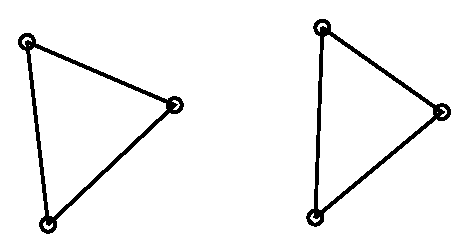
\includegraphics{tangled-cx}}
\caption{Tangled but non-connected graph}
\end{figure}
}

\ppart{8} 
An $n$-node graph is said to be {\em mangled} if there is an edge
leaving every set of $\lceil\frac{n}{2}\rceil$ or fewer vertices.
Again, as a special case, the graph consisting of a single node is
considered mangled.  Prove the following claim. \textit{Hint: Prove by contradiction.}

\bigskip

{\bf Claim.} Every non-empty, mangled graph is connected.

\solution{
The proof is by contradiction.  Assume for the purpose of
contradiction that these exists an $n$-node graph that is mangled, but
not connected.  Then the graph must have at least two connected
components.  However, there can be at most one connected component
with more than $\lceil\frac{n}{2}\rceil$ vertices, since the graph has
only $n$ vertices in total.  Therefore, there exists a connected
component with $\lceil\frac{n}{2}\rceil$ or fewer vertices.  Since the
graph is mangled, there is an edge leaving this component.  But this
contradicts the definition of a connected component.
}

\eparts

\end{problem}
\instatements{\newpage}


%%%%%%%%%%%%%%%%%%%%%%%%%%%%%%%%%%%%%%%%
%%%%%%%%%%%%%%%%%%%%%%%%%%%%%%%%%%%%%%%%
% New problem

\begin{problem}{10} 
Let the nodes in a tournament be ranked
according to their outdegrees, that is, node $u$ is ranked less than or equal to $v$ iff $outdegree(u)\leq outdegree(v)$.
Prove that the sum of the
outdegrees of the $i$ lowest ranked nodes is at least $i(i-1)/2$.

\solution{
Consider the subgraph on the $i$ lowest ranked nodes. This represents a
tournament as well. So, the number of its edges is equal to $i(i-1)/2$.
Each of these edges  are counted in the sum of the outdegrees of these $i$ nodes in the original graph.
}
\end{problem}
\instatements{\vspace{0.3in}}

%%%%%%%%%%%%%%%%%%%%%%%%%%%%%%%%%%%%%%%%
%%%%%%%%%%%%%%%%%%%%%%%%%%%%%%%%%%%%%%%%
% From Spring08, Class Problems 13 Monday

\begin{problem}{10}
  A directed graph is \term{symmetric} if, whenever $x \rightarrow y$ is an
  edge, so is $y \rightarrow x$.

  Given any finite, symmetric web graph, let
\[
PR(x) \mathbin{::=} \frac{\text{out-degree($x$)}}{e},
\]
where $e$ is the total number of edges in the graph.  Show that this is a solution for the system of equations that are satisfied by the page rank as discussed in section 2 of lecture notes 9. 

\solution{
We need to prove that $PR(x)=outdegree(x)/e$ satisfies the system of equations
$$\forall x, \ PR(x) = \sum_{y \mbox{ s.t. } y \rightarrow x} \frac{PR(y)}{outdegree(y)}$$
together with
$$\sum_{x} PR(x) =1.$$

  We derive
\begin{eqnarray*}
\sum_{y \mbox{ s.t. } y \rightarrow x} \frac{PR(y)}{outdegree(y)}
&=& \sum_{y \mbox{ s.t. } y \rightarrow x} 
 \paren{\frac{1}{\text{out-degree($y$)}}}\paren{\frac{\text{out-degree($y$)}}{e}} \\
&=& \sum_{y \mbox{ s.t. } y \rightarrow x}  \frac{1}{e} \\
&=& \frac{\text{in-degree($x$)}}{e}\\
&=&  \frac{\text{out-degree($x$)}}{e} \mbox{ (by symmetry of the graph)}\\
&=& PR(x)
\end{eqnarray*}
and
$$\sum_{x} PR(x) = \sum_x \frac{\text{out-degree($x$)}}{e} = \frac{e}{e}=1.$$
}
\end{problem}
\instatements{\vspace{0.5in}}

%%%%%%%%%%%%%%%%%%%%%%%%%%%%%%%%%%%%%%%%
%%%%%%%%%%%%%%%%%%%%%%%%%%%%%%%%%%%%%%%%
% From Fall06, Pset 5

\begin{problem}{25}
Two students from Podunk University have a neat idea with which they
intend to beat out all of the top search engines! Their new product,
based on a simple web search algorithm called {\em Doodle},  uses
the following ranking algorithm:
$$Doodlerank(x) = \sum_{y \rightarrow x} Doodlerank(y)$$
(the Doodleranks are required to be greater than or equal to 0).
This is much nicer than Pagerank, since it gets rid of that silly
weighting scheme!

\bparts

\ppart {5}
Describe the set of possible settings of Doodlerank's for the
nodes in the following graphs.
\begin{enumerate}
\item The directed path of length $n$.

\solution{ The first node in the path must get Doodlerank 0, and so,
by induction on the number of nodes along the path, all nodes must
get Doodlerank 0. }

\item The directed cycle of length $n$.

\solution{ All nodes must get the same Doodlerank. }
\end{enumerate}

\ppart {5}
Give an example of a graph in which each node can reach any
other node, but for which the only way to assign weights so that the
Doodlerank equations are satisfied is so that the Doodlerank weights
are all zero!

\solution{An example of such a graph:

\begin{figure}[htp]
\begin{center}
\includegraphics[width=55mm]{pset5-x1tox3.jpg}
\end{center}
\end{figure}

By the definition of the Doodlerank, we get the following equations:
\begin{align*}
Doodlerank(x_1) & = Doodlerank(x_2) \\
Doodlerank(x_2) & = Doodlerank(x_1) + Doodlerank(x_3) \\
Doodlerank(x_3) & = Doodlerank(x_2)
\end{align*}

Substituting the equations, we get $Doodlerank(x_2) = 2 \times Doodlerank(x_2)$, so all of the Doodleranks must be equal to 0.

%If either $x_1$ or $x_3$ has Doodlerank strictly greater than 0,
%then $x_2$ must have  Doodlerank strictly greater than 0.  Then
%$x_1$ and $x_3$ must both have Doodlerank strictly greater than 0.
%So, $x_2$, which has Doodlerank $x_1+x_3$ has Doodlerank strictly
%greater than that of $x_1$ or $x_3$. But, the Doodlerank of $x_1$
%must be equal to that that of $x_2$, and similarly, the Doodlerank
%of $x_3$ must be equal to that that of $x_2$, so we have a
%contradiction.
}

\eparts

Ok,  the Podunk students are finally convinced that they have
to use the weighting scheme from Google -- that is, the equations
must satisfy
$$Doodlerank(x) = \sum_{y \rightarrow x} \frac{Doodlerank(y)}{outdegree(y)}$$
However, the Podunk students want to make their fortune by skipping any modification of the original graph. Unlike Pagerank, the sinks in Doodlerank are not made to point to any universal supernodes and maintain an outdegree of 0.

This scheme has also a major problem!

\bparts

\ppart {5} First show by induction that if any node $x$ is assigned Doodlerank 0, then any node $y$ that
can reach $x$ in a directed walk must also be assigned Doodlerank $0$.

\solution{
\begin{proof}
The proof is by induction on the length of the path. Suppose $x$ is assigned Doodlerank 0. Let $P(n)$ be the predicate that any node that can reach $x$ in a minimum of $n$ steps must have Doodlerank 0.

\textbf{Base Case}: $n=0$, the node is $x$ and has Doodlerank 0.

\textbf{Inductive Step}: Assume $P(n)$ is true. Let $y$ be any node that can read $x$ in a minimum of $n+1$ steps, where $\pi$ is the length $n+1$ shortest path from $y$ to $x$. Let $x'$ be the first node after $y$ on $\pi$. The shortest path from $x'$ to $x$ is length $n$, since any shorter path would contradict $\pi$ as the shortest path from $y$ to $x$. Therefore, we know by the induction hypothesis that $x'$ has Doodlerank 0.

We know $y$ contributes $Doodlerank(y)/outdegree(y)$ to $Doodlerank(x')$, so the only way for $Doodlerank(x')=0$ is for $Doodlerank(y)=0$. Thus, $P(n+1)$ is true and, since $x$ was an arbitrary node, we have shown that any node which can reach a node of Doodlerank 0 must also have Doodlerank 0.

\end{proof}
}

\ppart {10}
In the next set of problem parts we are going to show that any sink must be assigned Doodlerank 0. To do this, we are going to think of the Doodlerank equations as describing votes by nodes for each of their neighbors. We represent a vote by $x$ for $y$ as a weighted edge $x \rightarrow y$.

\begin{enumerate}

\item
Suppose $V$ is the set of all the nodes in the graph. Let $S$ by the set of sinks and $T=V-S$ the set of non-sinks. First show that the Doodlerank of a single node $x \in T$ (i.e. $outdegree(x)\geq 1$) must equal the sum of the weights on the outgoing edges of $x$.

\solution{ $Doodlerank(x) = \frac{Doodlerank(x)}{outdegree(x)} \cdot outdegree(x) = \sum_{\{x \rightarrow y | y \in V\}} \frac{Doodlerank(x)}{outdegree(x)}$. }

\vspace{0.2in}

\item
Next show the same property holds over the entire set of non-sinks $T$ by writing the sum of Doodleranks of nodes in $T$, $\sum_{x \in T} Doodlerank(x)$, as the sum of the weights of outgoing edges from all nodes $x \in T$ to nodes $y \in V$.

\solution{
\begin{align*}
\sum_{x \in T} Doodlerank(x) = \sum_{x \in T} \sum_{\{x \rightarrow y | y \in V\}} \frac{Doodlerank(x)}{outdegree(x)} = \sum_{\{x \rightarrow y | x \in T, y \in V \}} \frac{Doodlerank(x)}{outdegree(x)}
\end{align*}}

\vspace{0.2in}

\item
Finally, show that any sink must be assigned Doodlerank 0.

\textit{Hint: Transform the sum of Doodleranks of non-sink nodes in $T$, $\sum_{x \in T} Doodlerank(x)$, into a sum of Doodleranks of all nodes in $V$, $\sum_{y \in V} Doodlerank(y)$. Use this to show that the sum of Doodleranks of all sink nodes $z \in S$ must be 0.}

\solution{
\begin{align*}
\sum_{x \in T} Doodlerank(x) & = \sum_{\{x \rightarrow y | x \in T, y \in V \}} \frac{Doodlerank(x)}{outdegree(x)} & \text{(from part 2)} \\
 & = \sum_{y \in V} \sum_{\{x \rightarrow y | x \in T\}} \frac{Doodlerank(x)}{outdegree(x)} & \text{(by summing over $y$)} \\
 & = \sum_{y \in V} \sum_{x \rightarrow y} \frac{Doodlerank(x)}{outdegree(x)} & \text{(since $x \rightarrow y \implies x \in T$)} \\
 & = \sum_{y \in V} Doodlerank(y) & \text{(by definition of Doodlerank)}
\end{align*}

Since $T=V-S$, it must be the case that
\begin{align*}
\sum_{x \in T} Doodlerank(x) = \sum_{y \in V} Doodlerank(y) - \sum_{z \in S} Doodlerank(z)
\end{align*}
But $\sum_{x \in T} Doodlerank(x) = \sum_{y \in V} Doodlerank(y)$, so $\sum_{z \in S} Doodlerank(z)$ = 0.

Since the Doodleranks cannot be negative, it must follow that for every sink $z$, $Doodlerank(z)$ = 0.
}

\vspace{0.2in}

\item Finally, conclude that any node which can reach a sink must also
be assigned a Doodlerank of 0.  So it's not too likely that Podunk
U. is going to be hitting up these students for contributions
anytime soon!

\solution{ We have shown that sinks must be assigned Doodlerank 0,
and that any node which can reach a Doodlerank 0 node must also be
assigned Doodlerank 0. Note that we just did a proof by induction in
which the base case was harder than the inductive step! }

\end{enumerate}

\eparts

\end{problem}

%%%%%%%%%%%%%%%%%%%%%%%%%%%%%%%%%%%%%%%%
%%%%%%%%%%%%%%%%%%%%%%%%%%%%%%%%%%%%%%%%
%%%%%%%%%%%%%%%%%%%%%%%%%%%%%%%%%%%%%%%%

\iffalse

%%%%%%%%%%%%%%%%%%%%%%%%%%%%%%%%%%%%%%%%
%%%%%%%%%%%%%%%%%%%%%%%%%%%%%%%%%%%%%%%%
% From Spring08, Pset6

\begin{problem}{15}

  A $3$-bit string is a string made up of $3$ characters, each a $0$
  or a $1$.  Suppose you'd like to write out, in one string, all eight
  of the 3-bit strings in any convenient order.  For example, if you
  wrote out the $3$-bit strings in the usual order starting with
  000 001 010\dots, you could concatenate them together to get a
  length $3\cdot 8 = 24$ string that started 000001010\dots.

  But you can get a shorter string containing all eight $3$-bit
  strings by starting with 00010\dots.  Now $000$ is present as bits
  $1$ through $3$, $001$ is present as bits $2$ through $4$, $010$ is
  present as bits $3$ through $5$, \dots.

\bparts

\ppart {3} Take a few moments to see how short a string you can make that
contains every $3$-bit string as $3$ consecutive bits somewhere in it.
Explain why $10$ bits is the absolute minimum length for such a
string.

\solution{$0001110100$ does it with $10$ bits and you can't do better:
  there must be two bits to start and each additional bit can yield at
  most one new $3$-bit string.}

\begin{figure} [htbp]
\centerline{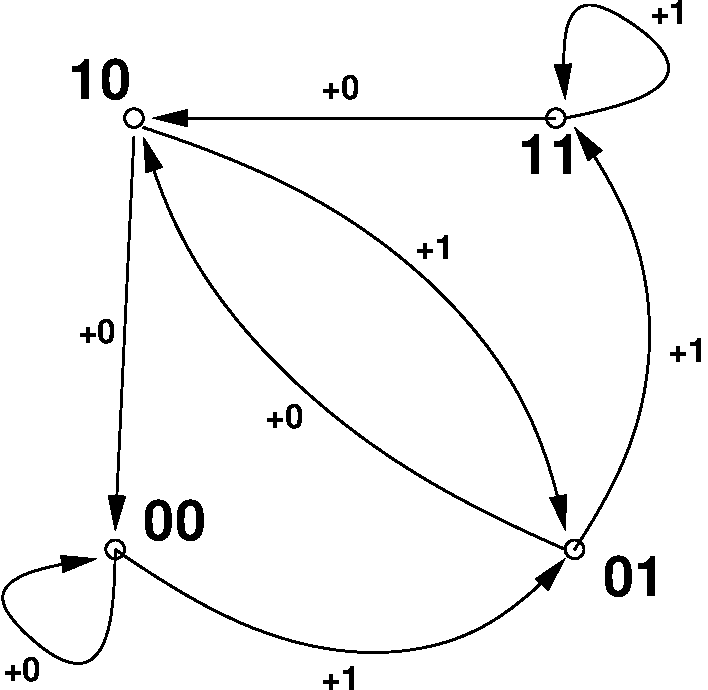
\includegraphics[width=2in]{debruijn}}
\end{figure}

\ppart {3} Imagine that the labels on the vertices of the directed graph above
represent the last two digits in a string you build by adding one bit
at a time.  Explain why the graph completely describes how
the last two digits of your string can change throughout this process.

\solution{No matter what the last two bits of your current string $x$
  are, say $ab$, there is a vertex representing that.  And, no matter
  what bit you want to use to extend $x$, say $c$, there is an edge
  directed from your current state, $ab$, to the vertex $bc$ that
  represents your new state, the last two bits of $xc$.  Furthermore,
  these are the only types of vertices and edges in the graph.  As a
  bonus, every edge $(s,s')$ is also labeled with the bit that was
  added to the string when going from the state $s$ to $s'$.}

\ppart {3} Find a directed path in this graph starting at some vertex, $v$,
that traverses every edge exactly once.  Note that vertices will have to
be used more than once and the path wil have to end in $v$.

\solution{Many: $00,00,01,11,11,10,01,10,00$ is one.}

\ppart {3} Explain how such a path provides a shortest possible solution
to the original problem.

\solution{Build a solution $x$ using the path.  Start with $x$ equal
  to the two digits in the label of the first vertex on the path.
  Then for every edge used after that, add on the bit labelling that
  edge to the string.  For example, the path given in last part's
  solution, yields the string $x=0001110100$.
  
  Since there are $8$ edges, the string will be of length $10$, the
  minimum possible.

  Furthermore, the label of the first vertex of the graph, followed by
  the label of the first edge, give the first $3$-bit substring in
  $x$. The next vertex and edge, give the next $3$-bit substring, and
  so on.  Since all possible $2$-bit vertex labels appear exactly
  once, and each vertex has a $1$ edge and a $0$ edge departing from
  it, every $3$-bit string corresponds to a unique vertex/out-edge
  combination.  The path uses every possible vertex/out-edge
  combination exactly once, so the string contains every $3$-bit
  sequence exactly once.}

\ppart  {3} What about $k$-bit substrings, $k = 4, 5, \ldots$?  Can you define the appropriate
generalization of the useful graph above?  (They're called de Bruijn
graphs.) If you do it sucessfully, you should be able to see that the
in-degree (as well as the out-degree) of every vertex is $2$.

\solution{
There are $2^k$ possible $k$-bit substrings. We can create $2^{k-1}$ nodes representing the different possible combinations of the first $k-1$ bits. The last bit will be represented as two edges out of each node (0 or 1) and two edges into each node (0 or 1).

It is a theorem that if the in-degree is equal to the out-degree at
every vertex of a digraph (and if the graph is connected when all the
edges are considered undirected edges) then a directed path can be
drawn in that digraph that uses every edge exactly once.  You might
want to think about why this should be true or how you might find such
a path.

But if you do believe it, you should be able to see why all $2^k$
$k$-bit strings can be written as substrings of a string of length
$2^k + k-1$.  (These strings are essentially de Bruijn strings.)}

\eparts

\end{problem}
\instatements{\newpage}

%%%%%%%%%%%%%%%%%%%%%%%%%%%%%%%%%%%%%%%%
%%%%%%%%%%%%%%%%%%%%%%%%%%%%%%%%%%%%%%%%
% From Spring07 Pset2

\begin{problem} {20}

An $n$-player \emph{tournament} consists of some set of $n\geq 2$
\emph{players}, and has the property that for every two players, $p \neq
q$, either $p$ beat $q$ or $q$ beat $p$, but not both.  \iffalse That is,
player $p$ beats player $q$ iff $q$ does not beat $p$, for all players $p
\neq q$.\fi

A sequence of distinct players $p_1,p_2, \ldots, p_k$, such that each
player beats the next one (that is, $p_i$ beats player $p_{i+1}$ for $1
\leq i < k$) is called a {\em ranking} of these players.  If also player
$p_k$ beats player $p_1$, the ranking is called a $k$-\emph{cycle}.

\begin{problemparts}

\ppart {10} Prove by induction that in every tournament, either there is a
``champion'' player that beats every other player, or there is a 3-cycle.

\solution{The induction hypothesis $P(n)$, is
``In an $n$-player tournament, either there is a player that
beats every other player, or there is a 3-cycle.''

\textbf{Base case} $n=2$: By definition of a 2-player tournament, one of the
players beats the only other player and therefore is the champion.

\textbf{Inductive step}:
Assume that $P(n)$ is true in order to show that $P(n+1)$ is true.

Consider an $n+1$-player tournament.  If there is a champion, we are done.
So we may assume that every player is beaten by some other player.  Now
remove any player, say player $p$, and treat the remaining $n$ players as an
$n$-player tournament.  There are two cases:

\begin{enumerate}

\item There is some champion in the $n$-player tournament who beats every
other player in the $n$-player tournament.

\item Every player in the $n$-player tournament is beaten by some other
player in the $n$-player tournament.

\end{enumerate}

\vspace{0.2in}
In case (1), there is some ``champion'', $q$, in the $n$-player tournament. We know:
\begin{itemize}
\item $p$ must beat $q$. (Everybody in the ($n+1$)-player tournament is beaten by somebody. Since $q$ is the champion in the $n$-player tournament, $q$ must be beaten by a player not in the $n$-player tournament, namely $p$.)
\item There exists some $r$ from the $n$-player tournament, where $r \neq q$, that beats $p$. (Everybody in the ($n+1$)-player tournament is beaten by somebody. By the rules of the tournament, $q$ cannot beat $p$, since we know $p$ beats $q$.)
\item $q$ must beat $r$. ($q$ is the champion in the $n$-player tournament.)
\end{itemize}
So we have found a 3-cycle $p,q,r$, proving $P(n+1)$.

\vspace{0.2in}
In case (2), we have by induction hypothesis a 3-cycle of players in the
$n$-player tournament. A 3-cycle in the $n$-player tournament will
also be a 3-cycle in the full $n+1$-player tournament, proving $P(n+1)$.

\vspace{0.2in}
}

\ppart {10} A {\em consistent ranking} is a sequence $p_1,p_2, \ldots,
p_n$ of all $n$ players in the tournament such that each player beats all
the later players in the sequence (that is, $p_i$ beats $p_j$ iff $i < j$,
for $1 \leq i,j \leq n$). Prove by induction, using the previous problem part, that a tournament has no consistent ranking \textit{iff} some subset of three of its players has no consistent ranking.

\solution{Since the statement is an ``iff" statement, we can rewrite the claim to say, ``A tournament has a consistent ranking \textit{iff} every subset of three of its players has a consistent ranking."

We first look at the forwards implication, that a tournament with a consistent ranking implies that every subset of three players has a consistent ranking. This is true by definition, since the relative rankings of any subset of two or more players in the tournaments are the same as in the entire tournament.

So we have only to prove the backwards implication, that if every subset of three players has a consistent ranking, then the tournament as a whole has one. The proof is by induction on $n$.

{\bf Base case $n=2$:} Every two player tournament obviously has a
consistent ranking.

{\bf Inductive step:} Suppose $n\geq 2$ and there is a consistent ranking
of any tournament of $n$ players whose three-player subsets have
consistent rankings.  Now consider any ($n+1$)-player tournament whose
three-player subsets have consistent rankings.

A three-player subset has a consistent ranking iff it does not form a 3-cycle. Since every three-player subset has a consistent ranking in the ($n+1$)-tournament, the ($n+1$)-tournament cannot have a 3-cycle. Hence, by the previous problem part, the tournament has a champion.

Suppose we remove the champion from the tournament. The $n$-player tournament that results also has no 3-cycles, since removing a node and its incident edges cannot form a cycle where there was none. Therefore, every subset of three players in the $n$-player tournament has a consistent ranking, and by induction, the entire $n$-player tournament has a consistent ranking.

Finally, in the ($n+1$)-player tournament, the champion followed by the ranking of $n$-nonchampions is a consistent ranking of all $n+1$ players.}

\end{problemparts}

\end{problem}

\fi

%%%%%%%%%%%%%%%%%%%%%%%%%%%%%%%%%%%%%%%%
%%%%%%%%%%%%%%%%%%%%%%%%%%%%%%%%%%%%%%%%
%%%%%%%%%%%%%%%%%%%%%%%%%%%%%%%%%%%%%%%%



\end{document}
